\documentclass{standalone}
\usepackage{tikz}

\usetikzlibrary{shapes.geometric}
\begin{document}
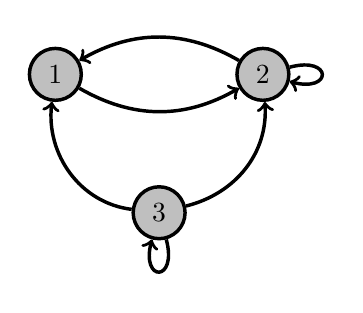
\begin{tikzpicture}
[every node/.style={inner sep=0pt}]
\node (3) [circle, minimum size=18.75pt, fill=lightgray, line width=1.25pt, draw=black] at (75.0pt, -75.0pt) {\textcolor{black}{3}};
\node (2) [circle, minimum size=18.75pt, fill=lightgray, line width=1.25pt, draw=black] at (112.5pt, -25.0pt) {\textcolor{black}{2}};
\node (1) [circle, minimum size=18.75pt, fill=lightgray, line width=1.25pt, draw=black] at (37.5pt, -25.0pt) {\textcolor{black}{1}};
\draw [line width=1.25, ->, color=black] (2) to  [in=30, out=150] (1);
\draw [line width=1.25, ->, color=black, loop right] (2) to (2);
\draw [line width=1.25, ->, color=black, loop below] (3) to (3);
\draw [line width=1.25, ->, color=black] (3) to  [in=274, out=14] (2);
\draw [line width=1.25, ->, color=black] (3) to  [in=263, out=173] (1);
\draw [line width=1.25, ->, color=black] (1) to  [in=210, out=330] (2);
\end{tikzpicture}

\end{document}
